\chapter{Aangeboren afweer en ontsteking}\label{ch:b3:innate-immunity}

Een splinter onder de huid brengt tienduizend bacteriën binnen die zich
elk half uur verdubbelen. Binnen minuten verwijden de vaten eromheen
zich en gaan zij lekken; binnen een uur hebben de eerste \omterm{def:b3:innate-immunity:innate}{neutrofielen}
zich uit het bloed geperst en kruipen zij langs een chemisch spoor naar
de indringers; binnen een dag is de plek rood, warm, gezwollen en
pijnlijk --- de vier tekenen van \omterm{def:b3:innate-immunity:inflammation}{ontsteking} die Celsus tweeduizend jaar
geleden opsomde --- en zijn de bacteriën dood, levend opgegeten door
cellen die hen als vreemd herkenden zonder hen ooit eerder te hebben
ontmoet. Dat is de \omterm{def:b3:innate-immunity:innate}{aangeboren afweer}: de verdediging die elk dier
heeft, klaar vóór de besmetting, in het genoom vastgelegd en niet
geleerd. Zij is snel, zij doodt de meeste indringers, en zij is wat de
tragere, geleerde afweer van het volgende hoofdstuk vertelt dat er iets
te leren valt. Haar uitwassen --- septische shock, chronische
\omterm{def:b3:innate-immunity:inflammation}{ontsteking}, de koortsen van auto-inflammatoire ziekten --- zijn even
leerzaam als haar successen.

\section{Lagen en cellen}

\begin{definition}[Aangeboren afweer]\label{def:b3:innate-immunity:innate}
\index{aangeboren afweer}\index{neutrofiel}\index{macrofaag}\index{dendritische cel}\index{natuurlijke doodcel}\index{barrière}
De \emph{aangeboren afweer} is het geheel van verdedigingen dat vóór
elke blootstelling aanwezig is, vastgelegd door kiembaangenen die zich
niet herschikken, dat geconserveerde kenmerken van microben herkent en
geen afzonderlijke individuen, dat binnen minuten tot uren werkt en
(met voorbehoud) zonder geheugen. Haar eerste laag zijn de
\emph{barrières}: het keratine van de huid, het slijm en de trilharen
van de luchtwegen, het zuur van de maag, het spoelen van urine en
tranen, het enzym lysozym dat \omterm{def:b3:bacteriology:envelope}{peptidoglycaan} knipt, de
\emph{antimicrobiële peptiden} (defensines, cathelicidines) die de
membranen van microben doorboren, en het commensale \omterm{def:b3:microbiomes:symbiosis}{microbioom} dat de
nissen bezet houdt (\cref{ch:b3:microbiomes}). Haar cellen, alle uit de
myeloïde lijn behalve de laatste: de \emph{neutrofielen}, \qty{60}{\%}
van de leukocyten van het bloed, $10^{11}$ per dag gemaakt, één dag
levend, de eerste die aankomen en de belangrijkste doders van
bacteriën; de \emph{macrofagen}, langlevende bewoners van elk weefsel
(kupffercellen in de lever, microglia in de hersenen, alveolaire
macrofagen in de long) die eten, opruimen en alarm slaan; de
\emph{dendritische cellen}, die weefsels bemonsteren en wat zij vinden
naar de lymfeknopen dragen; mestcellen, basofielen en eosinofielen,
gewapend tegen parasieten en verantwoordelijk voor allergie; en de
\emph{natuurlijke doodcellen} (NK-cellen), lymfocyten die besmette of
getransformeerde cellen op het eerste gezicht doden.
\end{definition}

\begin{proof}[Bewijsmateriaal]
Metchnikoff (1882) duwde in Messina een rozendoorn in een doorzichtige
zeesterlarve en zag de volgende ochtend beweeglijke cellen eromheen
samendrommen; hij had dezelfde cellen voedseldeeltjes en
kleurstofkorrels zien verzwelgen, en stelde voor dat zij ook microben
verzwolgen --- \emph{fagocyten}, de handhavers van een afweer die hij
daarna in elk dier opspoorde dat hij kon vinden, van amoeben tot de
mens. Hij deelde de Nobelprijs van 1908 met Ehrlich, wiens antilichamen
de tegenovergestelde, humorale opvatting vertegenwoordigden; beiden
hadden gelijk, en een eeuw later bleken de twee helften van de afweer
één systeem, waarin de aangeboren helft de adaptieve onderwijst.
\end{proof}

\begin{omfigure}
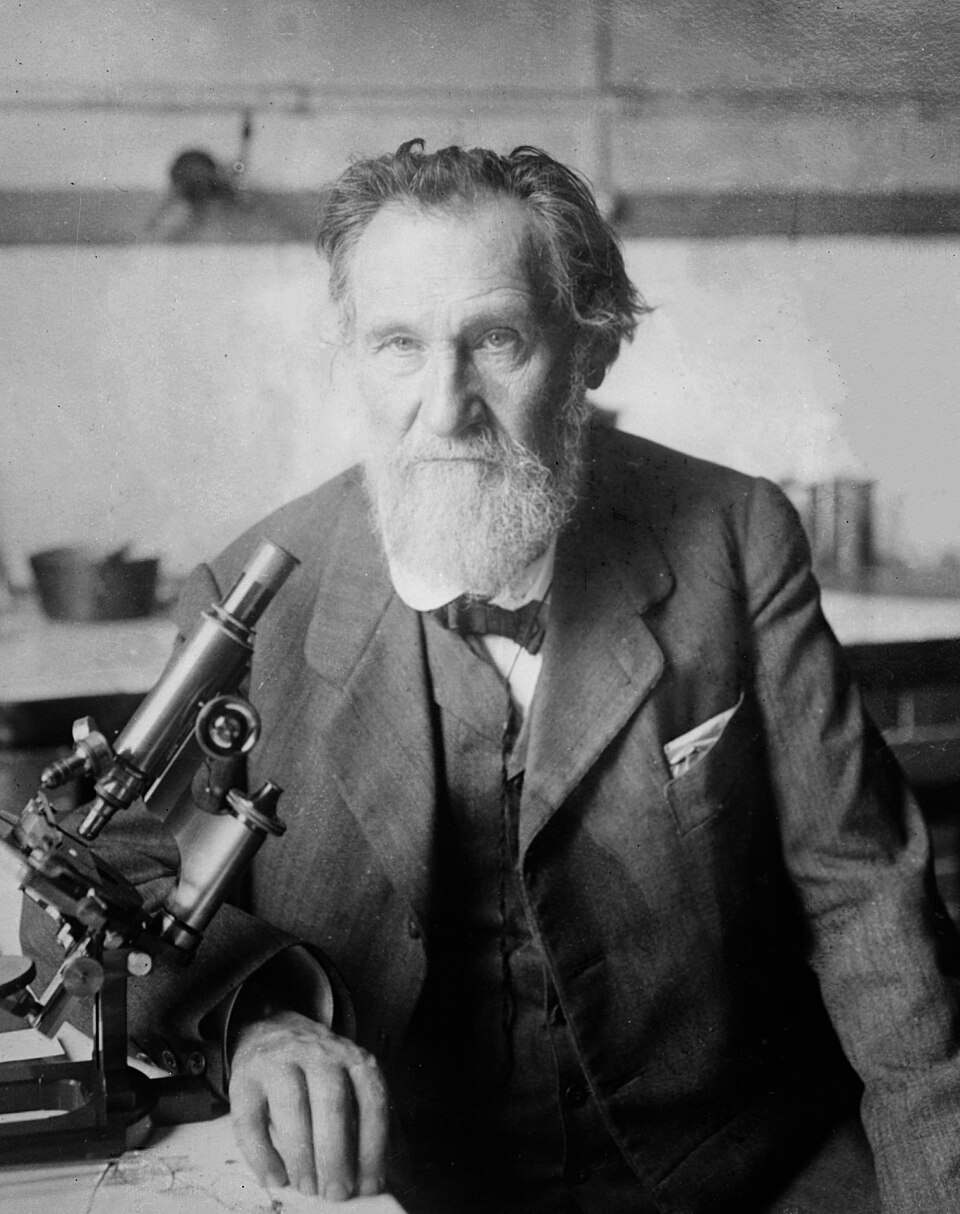
\includegraphics[width=0.30\linewidth]{images/book5/metchnikoff.jpg}\hspace{0.04\linewidth}
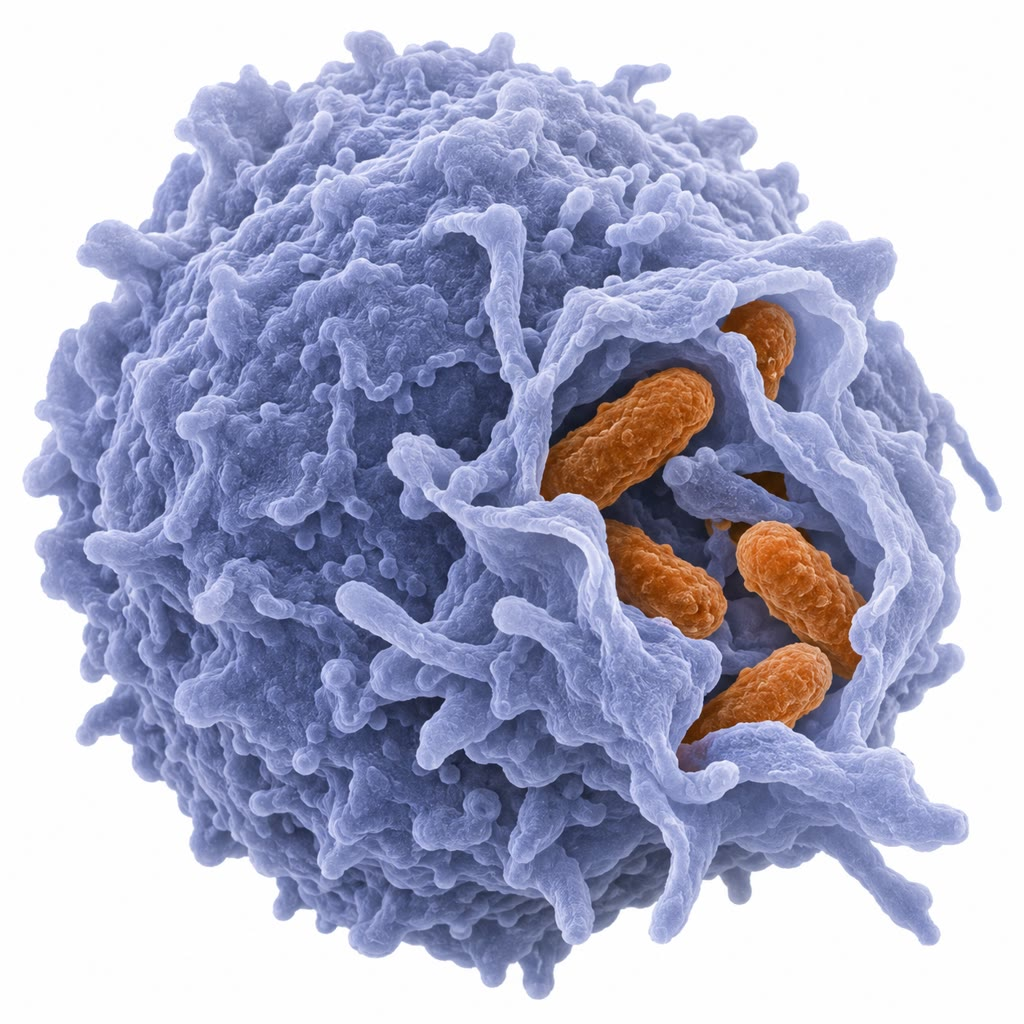
\includegraphics[width=0.30\linewidth]{images/book5/ai/b5-15-neutrophil-phagocytosis.jpg}\hspace{0.04\linewidth}
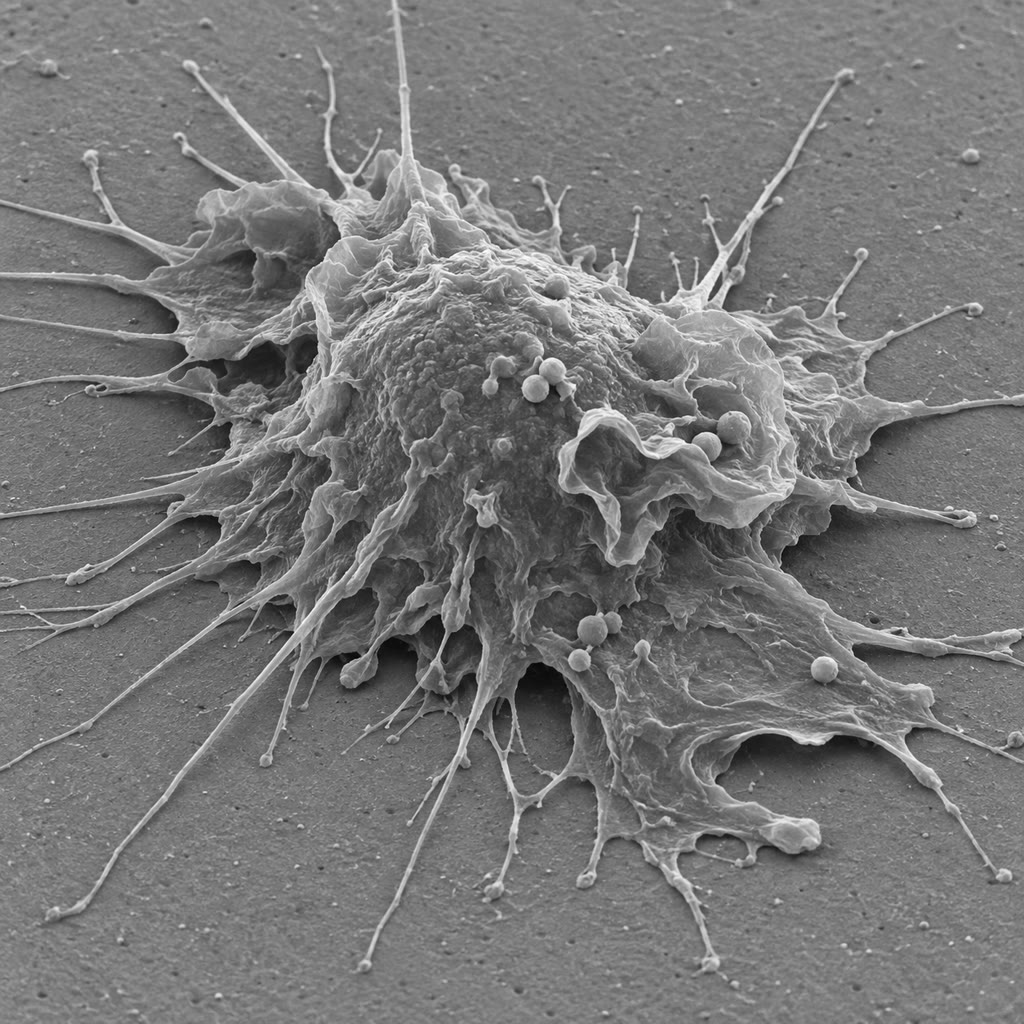
\includegraphics[width=0.30\linewidth]{images/book5/ai/b5-15-macrophage.jpg}

{\small Élie Metchnikoff, die fagocyten zag samendrommen rond een doorn
in een zeesterlarve en de cellulaire immunologie stichtte (Library of
Congress, publiek domein). Midden: een \omterm{def:b3:innate-immunity:innate}{neutrofiel} die bacteriën
verzwelgt. Rechts: een \omterm{def:b3:innate-immunity:innate}{macrofaag} die haar geplooide membranen over een
oppervlak uitspreidt.}
\end{omfigure}

\section{De vijand herkennen}

\begin{definition}[Patroonherkenning]\label{def:b3:innate-immunity:prr}
\index{patroonherkenningsreceptor}\index{met ziekteverwekkers verbonden moleculair patroon}\index{Toll-achtige receptor}\index{met schade verbonden moleculair patroon}\index{inflammasoom}
Cellen van de \omterm{def:b3:innate-immunity:innate}{aangeboren afweer} herkennen \emph{met ziekteverwekkers
verbonden moleculaire patronen} (PAMP's): moleculen die hele klassen
microben gemeen hebben, die voor hen onmisbaar zijn en die de gastheer
niet heeft --- \omterm{def:b3:bacteriology:envelope}{lipopolysacharide} van \omterm{def:b3:bacteriology:envelope}{gramnegatieve} wanden,
\omterm{def:b3:bacteriology:envelope}{peptidoglycaan} en lipoteichoïnezuur van \omterm{def:b3:bacteriology:envelope}{grampositieven}, flageline,
$\beta$-glucanen van schimmels, dubbelstrengs RNA, RNA zonder
5$'$-kap, DNA met ongemethyleerd \omterm{def:b3:chromatin-epigenetics:methylation}{CpG}, DNA in het cytosol. De receptoren
zijn \emph{patroonherkenningsreceptoren} (PRR's), enkele tientallen in
totaal, die elk door één gen worden vastgelegd: de \emph{Toll-achtige
receptoren} (TLR's) op het oppervlak en in endosomen (TLR4 voor
\omterm{def:b3:bacteriology:envelope}{lipopolysacharide}, TLR5 voor flageline, TLR3 voor dubbelstrengs RNA,
TLR9 voor CpG-DNA); de cytosolische NOD-eiwitten voor fragmenten van
\omterm{def:b3:bacteriology:envelope}{peptidoglycaan}, RIG-I voor viraal RNA, cGAS--STING voor cytosolisch
DNA; C-type-lectines voor schimmelsuikers. Dezelfde receptoren, of
andere uit dezelfde families, herkennen \emph{met schade verbonden
moleculaire patronen} (DAMP's) die door beschadigde cellen worden
vrijgelaten --- ATP, urinezuur, het kerneiwit HMGB1, mitochondriaal DNA
--- zodat ook steriele beschadiging ontsteekt. De binding activeert de
transcriptiefactoren NF-$\kappa$B en de regulerende factoren van het
interferon, die binnen een uur \omterm{def:b3:innate-immunity:inflammation}{cytokinen}, \omterm{def:b3:innate-immunity:inflammation}{chemokinen}, adhesiemoleculen
en antimicrobiële genen aanzetten; een deel van de cytosolische
sensoren stelt het \emph{inflammasoom} samen, een platform dat
caspase-1 activeert om interleukine-1$\beta$ in zijn werkzame vorm te
knippen en om de ontstekingsdood \omterm{def:b3:cell-cycle-apoptosis:other}{pyroptose} uit te lokken
(\cref{ch:b3:cell-cycle-apoptosis}).
\end{definition}

\begin{proof}[Bewijsmateriaal]
Janeway stelde in 1989 voor dat het adaptieve afweersysteem niet op
antigeen alleen reageert maar een signaal nodig heeft van aangeboren
receptoren die microbiële patronen hebben herkend --- de verklaring
waarom vaccins adjuvantia nodig hebben, ``het vuile geheimpje van de
immunoloog''. Hoffmann (1996) vond dat \emph{Drosophila} zonder de
receptor Toll, bekend van zijn rol bij de aanleg van het embryo, geen
afweer tegen schimmels op gang kon brengen en onder de schimmel
bedolven stierf; Beutler (1998) bracht de weerstand tegen
\omterm{def:b3:bacteriology:envelope}{lipopolysacharide} van een muizenstam, die doses endotoxine overleefde
die voor andere dodelijk waren en \omterm{def:b3:bacteriology:envelope}{gramnegatieve} infecties niet
opruimde, terug tot een mutatie in de homoloog bij zoogdieren, TLR4. De
receptor voor endotoxine, vijftig jaar lang gezocht, was een Toll.
\end{proof}

\begin{omfigure}
\begin{tikzpicture}[every node/.style={font=\scriptsize}, >=stealth]
  % membrane
  \draw[very thick, omDef] (0,3.0) -- (11.5,3.0); \draw[very thick, omDef] (0,2.7) -- (11.5,2.7);
  \node[above] at (0.5,3.05) {buiten}; \node[below] at (0.5,2.65) {cytosol};
  % TLR4 with LPS
  \draw[thick, fill=omProp!35] (2.2,2.4) rectangle (2.6,3.9); \draw[thick, fill=omProp!35] (2.9,2.4) rectangle (3.3,3.9);
  \fill[omThm] (2.75,4.1) circle (0.14); \node[above] at (2.75,4.25) {LPS (een PAMP)};
  \node[right, align=left] at (3.4,3.5) {TLR4-dimeer\\met MD2};
  % signalling
  \node[draw, thick, rounded corners, fill=omDef!20] (myd) at (2.75,1.7) {MyD88, kinasen};
  \node[draw, thick, rounded corners, fill=omDef!20] (nfkb) at (2.75,0.6) {NF-$\kappa$B vrijgemaakt};
  \node[draw, thick, rounded corners, fill=omMeth!25, align=center] (genes) at (2.75,-0.8) {TNF, IL-1$\beta$, IL-6, IL-8;\\adhesiemoleculen; iNOS};
  \draw[->, thick] (2.75,2.4) -- (myd); \draw[->, thick] (myd) -- (nfkb); \draw[->, thick] (nfkb) -- (genes);
  \node[right, font=\tiny] at (3.3,1.2) {binnen een uur};
  % cytosolic sensors
  \node[draw, thick, rounded corners, fill=omProp!25, align=center] (rig) at (6.9,1.9) {RIG-I: viraal RNA\\cGAS--STING: cytosolisch DNA};
  \node[draw, thick, rounded corners, fill=omMeth!25] (ifn) at (6.9,-0.2) {type-I-interferon};
  \draw[->, thick] (rig) -- node[midway, right] {IRF3, IRF7} (ifn);
  \node[draw, thick, rounded corners, fill=omThm!20, align=center] (nlrp) at (10.9,1.9) {NLRP3-inflammasoom:\\kristallen, ATP, poriën};
  \node[draw, thick, rounded corners, fill=omMeth!25, align=center] (il1) at (10.9,-0.8) {caspase-1: IL-1$\beta$\\vrijgemaakt; pyroptose};
  \draw[->, thick] (nlrp) -- (il1);
  \draw[->, thick, dashed] (genes.south) -- ++(0,-0.5) -| (il1.south) node[pos=0.25, below, font=\tiny] {pro-IL-1$\beta$ geleverd door de TLR-route};
\end{tikzpicture}

{\small Drie armen van de patroonherkenning. Een \omterm{def:b3:innate-immunity:prr}{Toll-achtige receptor}
aan het oppervlak, gebonden door \omterm{def:b3:bacteriology:envelope}{lipopolysacharide}, geeft via
NF-$\kappa$B door aan de ontstekingscytokinen; cytosolische sensoren van
viraal nucleïnezuur zetten interferon aan; het \omterm{def:b3:innate-immunity:prr}{inflammasoom} maakt van
de opgeslagen voorloper van interleukine-1 het werkzame \omterm{def:b3:innate-immunity:inflammation}{cytokine}.}
\end{omfigure}

\begin{definition}[Complement]\label{def:b3:innate-immunity:complement}
\index{complement}\index{C3-convertase}\index{opsonisatie}\index{membraanaanvalscomplex}\index{anafylatoxine}
Het \emph{complement} is een systeem van zo'n dertig plasma-eiwitten,
\qty{10}{\%} van de serumglobulines, dat microben met een cascade van
proteolytische activeringen merkt en vernietigt. Drie routes komen
samen op het knippen van het centrale eiwit C3: de \emph{klassieke}
route, gestart doordat C1q antilichamen op een oppervlak bindt (of
\omterm{prop:b3:innate-immunity:systemic}{C-reactief eiwit}, of apoptotische cellen); de \emph{lectineroute},
gestart doordat mannosebindend lectine microbiële suikers herkent; en
de \emph{alternatieve} route, waarin C3 spontaan met lage snelheid
hydrolyseert en het C3b dat daarbij ontstaat zich aan elk oppervlak
hecht dat het tegenkomt. Elke route bouwt een \emph{C3-convertase}, een
enzym dat meer C3 knipt; het C3b dat het covalent op het oppervlak
neerlegt bouwt op zijn beurt meer convertase --- een versterkingslus
--- zodat een bacterie binnen minuten met miljoenen C3b is bedekt. C3b
is een \emph{opsonine}: fagocyten dragen er receptoren voor en eten wat
het bedekt. De kleine fragmenten C3a en C5a zijn
\emph{anafylatoxinen} die vaten verwijden, \omterm{def:b3:innate-immunity:innate}{neutrofielen} aantrekken en
mestcellen activeren. En C5b stelt C6--C9 samen tot het
\emph{membraanaanvalscomplex}, een porie van \qty{10}{nm} die
\omterm{def:b3:bacteriology:envelope}{gramnegatieve} bacteriën en virussen met \omterm{def:b3:virology:virus}{envelop} doet uiteenvallen.
Gastheercellen worden gespaard omdat zij regulatoren dragen ---
factor~H, CD55, CD59 --- die het convertase op hun eigen oppervlak
uiteenhalen en de porie blokkeren; microben, die ze missen, worden door
de lus verteerd.
\end{definition}

\begin{theorem}[De complementlus als kinetische scheidsrechter]\label{thm:b3:innate-immunity:complement}
\index{complement!versterkingslus}
Zij $B(t)$ het aantal C3b-moleculen dat op een oppervlak is neergelegd.
C3b wordt met een kleine constante snelheid $k_{0}$ neergelegd uit het
langzame doorlopen van C3, en elk neergelegd C3b bouwt convertase dat
er met snelheid $a$ per C3b per seconde meer neerlegt, terwijl
regulatoren (bij de gastheer) en verval de convertase-activiteit met
snelheid $d$ per C3b per seconde weghalen:
\[
\frac{\mathrm{d}B}{\mathrm{d}t} = k_{0} + (a - d)\,B .
\]
Op een oppervlak waar $a > d$ --- een microbe, zonder regulatoren ---
groeit $B(t) = \bigl[k_{0}/(a-d)\bigr]\bigl(e^{(a-d)t} - 1\bigr)$
exponentieel met tijdconstante $1/(a - d)$; op een gastheeroppervlak
waar $d > a$ nadert $B$ de kleine evenwichtswaarde $k_{0}/(d - a)$.
Dezelfde moleculen leggen bij dezelfde concentraties in enkele minuten
een miljoen C3b op een bacterie neer en enkele tientallen op de cel
ernaast: het onderscheid tussen eigen en vreemd wordt niet door
herkenning gemaakt maar door het teken van $a - d$.
\end{theorem}
\begin{proof}
De vergelijking is lineair met constante coëfficiënten. Voor $a \ne d$
is het vaste punt $B^{*} = -k_{0}/(a-d)$; met $B = B^{*} + u$ geldt
$\mathrm{d}u/\mathrm{d}t = (a-d)u$, dus $u = u_{0}e^{(a-d)t}$, en met
$B(0) = 0$ is $B(t) = \bigl[k_{0}/(a-d)\bigr](e^{(a-d)t} - 1)$. Voor
$a > d$ groeit dit onbegrensd (tot het C3 of het oppervlak opraakt);
voor $a < d$ dooft de exponentiële uit en gaat $B \to k_{0}/(d-a) > 0$.
Met $k_{0} = 1$ per seconde en $a - d = \qty{0.1}{s^{-1}}$ op een
bacterie is $B(\qty{2}{min})
= 10(e^{12} - 1) \approx 1.6\times 10^{6}$; met $d - a =
\qty{0.1}{s^{-1}}$ op een gastheercel is $B^{*} = 10$.
\end{proof}

\begin{omfigure}
\begin{tikzpicture}
\begin{axis}[
  width=0.66\linewidth, height=5.6cm,
  axis x line=bottom, axis y line=left,
  xmin=0, xmax=150, ymin=1, ymax=1e7, ymode=log,
  xlabel={seconden}, ylabel={neergelegd C3b},
  xlabel style={font=\small, at={(axis description cs:0.5,-0.12)}, anchor=north}, ylabel style={font=\small},
  tick label style={font=\small}, xtick={0,30,60,90,120,150},
  clip=false,
]
\addplot[very thick, omThm, domain=1:150, samples=80] {10*(exp(0.1*x)-1)};
\addplot[very thick, omDef, domain=1:150, samples=80] {10*(1-exp(-0.1*x))};
\node[font=\scriptsize, omThm, anchor=east] at (axis cs:100,2e5) {microbe: $a > d$, exponentieel};
\node[font=\scriptsize, omDef, anchor=south west] at (axis cs:60,14) {gastheercel: $d > a$, verzadigt bij $k_{0}/(d-a)$};
\end{axis}
\end{tikzpicture}

{\small De complementlus op twee oppervlakken met $k_{0} = 1$ per
seconde en $|a - d| = \qty{0.1}{s^{-1}}$: op een microbe zonder
regulatoren groeit C3b exponentieel en haalt het in twee minuten een
miljoen; op een gastheercel met regulatoren vlakt het af bij tien.}
\end{omfigure}

\begin{omfigure}
\begin{tikzpicture}[every node/.style={font=\scriptsize}, >=stealth]
  \node[draw, thick, rounded corners, fill=omDef!20, align=center] (cl) at (-4.2,3.0) {klassiek:\\C1q op antilichaam\\of C-reactief eiwit};
  \node[draw, thick, rounded corners, fill=omDef!20, align=center] (le) at (0,3.0) {lectine:\\mannosebindend lectine\\op microbiële suikers};
  \node[draw, thick, rounded corners, fill=omDef!20, align=center] (al) at (4.2,3.0) {alternatief:\\spontaan doorlopen van C3,\\C3b op elk oppervlak};
  \node[draw, thick, rounded corners, fill=omProp!35, minimum width=3cm] (conv) at (0,1.2) {C3-convertase};
  \node[draw, thick, rounded corners, fill=omThm!25, align=center] (c3b) at (0,-0.4) {C3 $\to$ C3b (op het oppervlak) $+$ C3a};
  \draw[->, thick] (cl) -- (conv); \draw[->, thick] (le) -- (conv); \draw[->, thick] (al) -- (conv);
  \draw[->, thick] (conv) -- (c3b);
  \draw[->, very thick, omThm] (c3b.east) .. controls (3.2,-0.4) and (3.2,1.2) .. (conv.east) node[pos=0.5, right, align=left] {versterkingslus:\\C3b bouwt meer convertase};
  \node[draw, thick, rounded corners, fill=omMeth!25, align=center] (ops) at (-4.4,-2.2) {opsonisatie:\\fagocyten eten\\wat C3b bedekt};
  \node[draw, thick, rounded corners, fill=omMeth!25, align=center] (ana) at (0,-2.2) {C3a, C5a:\\vaten verwijden, neutrofielen\\en mestcellen aangetrokken};
  \node[draw, thick, rounded corners, fill=omMeth!25, align=center] (mac) at (4.4,-2.2) {C5b--C9:\\membraanaanvalscomplex,\\uiteenvallen};
  \draw[->, thick] (c3b) -- (ops); \draw[->, thick] (c3b) -- (ana); \draw[->, thick] (c3b) -- (mac);
  \node[draw, thick, rounded corners, fill=gray!15, align=center] (reg) at (-4.4,1.2) {regulatoren van de gastheer:\\factor~H, CD55, CD59};
  \draw[-|, thick, gray!60!black] (reg) -- (conv);
\end{tikzpicture}

{\small \omterm{def:b3:innate-immunity:complement}{Complement}. Drie wegen bouwen een \omterm{def:b3:innate-immunity:complement}{C3-convertase}; het C3b dat
het neerlegt bouwt er meer (de lus van de stelling), en het neergelegde
C3b opsoniseert, de fragmenten ontsteken, en het eindcomplex doet de
cel uiteenvallen. Gastheercellen dragen regulatoren die de lus
doorsnijden (en, met CD59, de porie blokkeren) op hun eigen membranen.}
\end{omfigure}

\section{Ontsteking}

\begin{definition}[Acute ontsteking]\label{def:b3:innate-immunity:inflammation}
\index{ontsteking}\index{cytokine}\index{chemokine}\index{extravasatie}\index{selectine}\index{integrine}
De \emph{ontsteking} is het antwoord van doorbloed weefsel op
beschadiging of besmetting, geregisseerd door \emph{cytokinen} --- de
kleine signaaleiwitten van afweercellen, hier vooral TNF,
interleukine-1 en interleukine-6 van geactiveerde \omterm{def:b3:innate-immunity:innate}{macrofagen} --- en
door \emph{chemokinen}, de cytokinen die de migratie sturen. Haar
stappen verklaren de tekenen van Celsus. Histamine uit mestcellen,
stikstofmonoxide en prostaglandines verwijden de arteriolen: de
\emph{roodheid} en de \emph{warmte}. Het endotheel van de venulen trekt
samen en laat plasma door, waarvan de eiwitten --- \omterm{def:b3:innate-immunity:complement}{complement},
antilichamen, stollingsfactoren --- het weefsel overspoelen: de
\emph{zwelling}. Bradykinine en prostaglandine E$_{2}$ maken de
zenuwuiteinden gevoelig: de \emph{pijn}. En de leukocyten komen aan
door \emph{extravasatie}: TNF en interleukine-1 laten het endotheel
\emph{selectines} tonen, waarop voorbijkomende \omterm{def:b3:innate-immunity:innate}{neutrofielen} haken en
rollen; chemokinen (interleukine-8) op het endotheeloppervlak
activeren de \emph{integrines} van de \omterm{def:b3:innate-immunity:innate}{neutrofielen}, die stevig aan
adhesiemoleculen van het endotheel binden en de cel stilzetten; en de
\omterm{def:b3:innate-immunity:innate}{neutrofiel} wringt zich tussen de endotheelcellen door en volgt de
chemokinegradiënt het weefsel in --- de hele reeks in enkele minuten,
tot een miljoen cellen per uur naar een besmette plek.
\end{definition}

\begin{omfigure}
\begin{tikzpicture}[every node/.style={font=\scriptsize}, >=stealth]
  % vessel wall
  \fill[omThm!10] (0,0) rectangle (12,2.3); \node[left, omThm!70!black, anchor=north east] at (12,2.25) {bloed, stroomt $\rightarrow$};
  \foreach \x in {0,1.5,3,4.5,6,7.5,9,10.5} \draw[thick, fill=omDef!30] (\x,-0.05) rectangle (\x+1.45,0.35);
  \node[right] at (0.1,-0.35) {endotheel};
  \fill[omMeth!8] (0,-1.7) rectangle (12,-0.45); \node[right, omMeth!60!black] at (0.1,-1.55) {weefsel};
  % bacteria and chemokine gradient
  \foreach \p in {(10.6,-1.1),(11.0,-0.9),(11.3,-1.2)} \fill[omProp] \p ellipse (0.14 and 0.07);
  \node[below, omProp] at (11.0,-1.35) {bacteriën};
  \node[below, font=\tiny] at (8.0,-0.5) {chemokinegradiënt $\rightarrow$};
  % neutrophils in sequence
  \draw[thick, fill=white] (1.2,1.1) circle (0.3); \node[above] at (1.2,1.45) {1. stroomt mee};
  \draw[thick, fill=white] (3.4,0.68) circle (0.3); \node[above] at (3.4,1.05) {2. rolt op selectines};
  \draw[omThm, thick] (3.1,0.45) -- (3.05,0.35); \draw[omThm, thick] (3.4,0.38) -- (3.4,0.35); \draw[omThm, thick] (3.7,0.45) -- (3.75,0.35);
  \draw[thick, fill=white] (6.0,0.62) ellipse (0.38 and 0.26); \node[above, align=center] at (6.0,0.95) {3. vaste hechting\\(integrines)};
  \draw[thick, fill=white] (8.25,0.18) ellipse (0.2 and 0.42); \node[above, align=center] at (8.4,0.95) {4. wringt zich\\erdoor};
  \draw[thick, fill=white] (9.6,-1.0) circle (0.3); \node[left] at (9.25,-1.0) {5. kruipt naar de plek};
  \draw[->, thick, gray] (1.5,1.05) -- (3.0,0.8); \draw[->, thick, gray] (3.7,0.68) -- (5.6,0.62); \draw[->, thick, gray] (6.4,0.5) -- (8.0,0.4); \draw[->, thick, gray] (8.3,-0.3) -- (9.3,-0.8);
  % TNF label
  \node[below, align=center, font=\tiny] at (4.0,-1.75) {TNF en IL-1 uit macrofagen in het weefsel laten het endotheel\\de selectines en adhesiemoleculen tonen die de neutrofielen vangen};
\end{tikzpicture}

{\small \omterm{def:b3:innate-immunity:inflammation}{Extravasatie}. \omterm{def:b3:innate-immunity:inflammation}{Cytokinen} uit \omterm{def:b3:innate-immunity:innate}{macrofagen} in het weefsel maken de
venulewand kleverig; een voorbijkomende \omterm{def:b3:innate-immunity:innate}{neutrofiel} haakt aan \omterm{def:b3:innate-immunity:inflammation}{selectines}
en rolt, wordt door zijn \omterm{def:b3:innate-immunity:inflammation}{integrines} stilgezet, wringt zich tussen de
endotheelcellen door, en volgt de chemokinegradiënt naar de bacteriën.}
\end{omfigure}

\begin{proposition}[Koorts, de acutefasereactie en de oplossing]\label{prop:b3:innate-immunity:systemic}
\index{koorts}\index{acutefasereactie}\index{C-reactief eiwit}\index{oplossing van de ontsteking}
Interleukine-1, TNF en interleukine-6 werken ook op afstand. In de
hypothalamus zetten zij prostaglandine E$_{2}$ aan, dat het instelpunt
van de lichaamstemperatuur verhoogt: de \emph{koorts}, die veel
bacteriën vertraagt, de eigen reacties van de afweercellen versnelt, en
per graad ongeveer \qty{12}{\%} meer stofwisseling kost. In de lever
zetten zij de \emph{acutefase-eiwitten} aan --- het C-reactieve eiwit,
dat bacterieel fosfocholine bindt en het \omterm{def:b3:innate-immunity:complement}{complement} activeert en dat
binnen twee dagen duizendvoudig stijgt, de maat van de \omterm{def:b3:innate-immunity:inflammation}{ontsteking} voor
de arts; fibrinogeen; mannosebindend lectine; en hepcidine, dat het
ijzer wegsluit voor de microben die het nodig hebben. In het beenmerg
laten zij \omterm{def:b3:innate-immunity:innate}{neutrofielen} los en versnellen zij hun aanmaak. Een
\omterm{def:b3:innate-immunity:inflammation}{ontsteking} is bedoeld om te eindigen: naarmate de prikkel is opgeruimd
gaan de lipidebemiddelaars van prostaglandines over op lipoxines en
resolvines, sterven \omterm{def:b3:innate-immunity:innate}{neutrofielen} door \omterm{def:b3:cell-cycle-apoptosis:apoptosis}{apoptose} en worden zij door
\omterm{def:b3:innate-immunity:innate}{macrofagen} opgegeten, die daarna op een herstelprogramma overgaan en
groeifactoren en interleukine-10 uitscheiden --- de \emph{oplossing}.
Houdt de prikkel aan (een tuberkelbacil die niet te doden is, een
kristal, een lichaamseigen antigeen), dan wordt de reactie chronisch:
\omterm{def:b3:innate-immunity:innate}{macrofagen} muren de plek in een granuloom in, fibroblasten leggen
littekenweefsel aan, en het weefsel wordt door zijn eigen verdediging
vernield.
\end{proposition}

\begin{example}[Sepsis]\label{ex:b3:innate-immunity:sepsis}
Een \omterm{def:b3:innate-immunity:inflammation}{ontsteking} die tot een splinter beperkt blijft is een genezing;
dezelfde reacties door het hele lichaam zijn een ramp. Wanneer
bacteriën of hun \omterm{def:b3:bacteriology:envelope}{lipopolysacharide} in hoeveelheid het bloed bereiken,
laten \omterm{def:b3:innate-immunity:innate}{macrofagen} overal tegelijk TNF en interleukine-1 los: elk vat
verwijdt zich en gaat lekken, de bloeddruk stort in, de stolling wordt
in tienduizend haarvaten geactiveerd en verbruikt de stollingsfactoren,
en de organen begeven het bij gebrek aan doorbloeding --- de
\emph{septische shock}, die een kwart tot de helft van wie zij treft
doodt, zo'n elf miljoen mensen per jaar. Enkele microgrammen
\omterm{def:b3:bacteriology:envelope}{lipopolysacharide} in een vrijwilliger gespoten geven binnen twee uur
koorts, koude rillingen en een daling van de bloeddruk; een muis zonder
TLR4 trekt zich niets aan van een dosis die honderd keer dodelijk is.
De ziekte is de reactie van de gastheer, en de \omterm{def:b3:bacteriology:antibiotics}{antibiotica} die de
bacteriën doden kunnen haar enkele uren lang verergeren door meer
endotoxine vrij te maken.
\end{example}

\begin{omfigure}
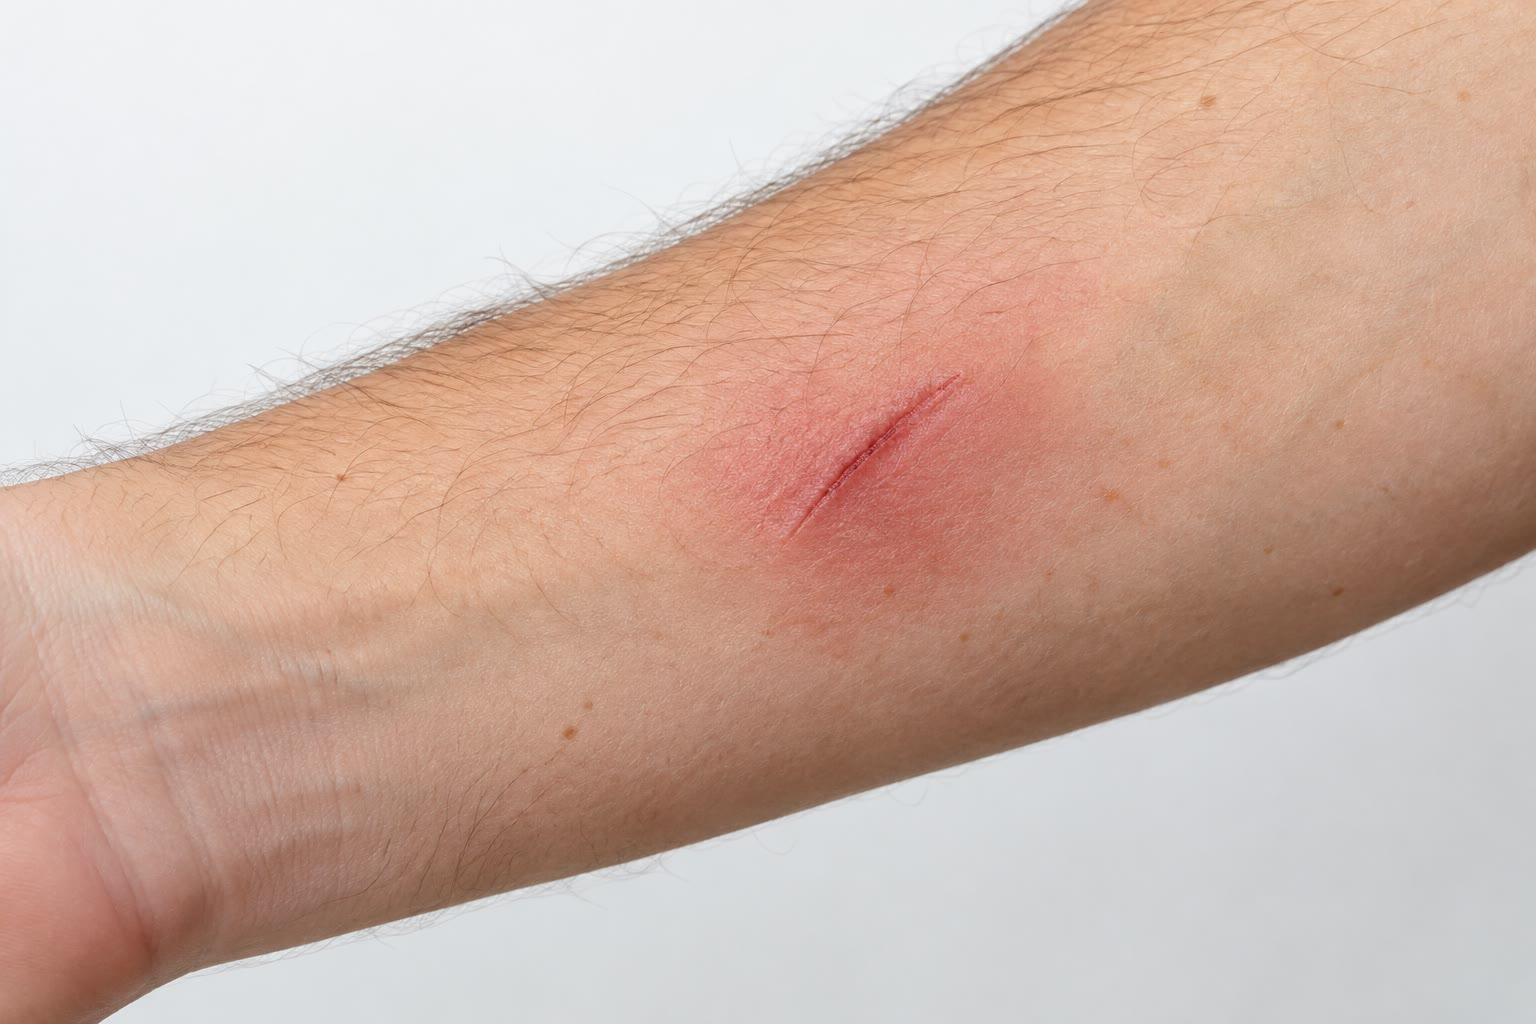
\includegraphics[width=0.52\linewidth]{images/book5/ai/b5-15-inflamed-skin.jpg}

{\small Acute \omterm{def:b3:innate-immunity:inflammation}{ontsteking} rond een schram van een doorn: roodheid en
warmte door verwijde vaten, zwelling door gelekt plasma, en de pijn die
het lidmaat stil houdt --- de plaatselijke reactie die, over het hele
lichaam veralgemeend, de septische shock is.}
\end{omfigure}

\section{Doden}

\begin{definition}[Fagocytose en de ademhalingsuitbarsting]\label{def:b3:innate-immunity:killing}
\index{fagocytose}\index{ademhalingsuitbarsting}\index{NADPH-oxidase}\index{extracellulair net van neutrofielen}
Een fagocyt bindt zijn prooi via receptoren voor opsoninen --- C3b en
de constante gebieden van antilichamen --- of rechtstreeks via
patroonreceptoren, wikkelt haar in membraan, en sluit het
\emph{fagosoom}, dat met granules en lysosomen versmelt. Het doden
gebeurt op verscheidene manieren tegelijk. De
\emph{ademhalingsuitbarsting}: het enzym \emph{NADPH-oxidase}, op het
fagosoommembraan samengesteld, pompt elektronen op zuurstof en maakt zo
superoxide, dat waterstofperoxide wordt, dat het myeloperoxidase met
chloride in hypochloriet omzet --- bleekmiddel, in millimolaire
concentratie binnen een compartiment van een micrometer. Verder
stikstofmonoxide van het induceerbare NO-synthase, dat met superoxide
peroxynitriet geeft. Zuur, tot pH~5. Lysozym, proteasen, lactoferrine
dat de prooi van ijzer berooft, en defensines die haar doorboren. Een
\omterm{def:b3:innate-immunity:innate}{neutrofiel} die niet kan opeten wat hij vindt --- een schimmeldraad, een
klont --- kan zijn eigen \omterm{def:b3:chromatin-epigenetics:nucleosome}{chromatine} als een kleverig net van DNA en
granule-eiwitten uitwerpen, een \emph{extracellulair net van
\omterm{def:b3:innate-immunity:innate}{neutrofielen}}, en daarbij sterven. Kinderen die een gebrekkig
NADPH-oxidase erven (chronische granulomateuze ziekte) krijgen telkens
terugkerende abcessen en granulomen door bacteriën en schimmels die
gewone fagocyten moeiteloos doden: de uitbarsting is niet
vrijblijvend.
\end{definition}

\begin{definition}[Natuurlijke doodcellen en interferon]\label{def:b3:innate-immunity:nk-ifn}
\index{natuurlijke doodcel!ontbrekend eigen}\index{interferon!type I}\index{antivirale toestand}
Virussen verschuilen zich in cellen, waar het \omterm{def:b3:innate-immunity:complement}{complement} en de fagocyten
niet bij hen kunnen. \emph{\omterm{def:b3:innate-immunity:innate}{Natuurlijke doodcellen}} speuren naar cellen
die MHC klasse~I niet meer tonen --- het ``ontbrekende eigen'' van een
cel waarvan de virale of tumorale bewoner de antigeenpresentatie heeft
uitgezet om aan de T-cellen te ontsnappen
(\cref{ch:b3:adaptive-immunity}) --- en naar stresseiwitten die besmette
en getransformeerde cellen op hun oppervlak zetten; remmende receptoren
voor MHC~I en activerende receptoren voor de stressliganden worden
opgeteld, en een cel die de balans doet omslaan wordt binnen minuten
gedood door perforine en granzymen die in haar worden gespoten en haar
\omterm{def:b3:cell-cycle-apoptosis:apoptosis}{apoptose} in gang zetten. \emph{Type-I-interferonen} ($\alpha$ en
$\beta$) worden gemaakt door elke cel waarvan RIG-I of cGAS viraal
nucleïnezuur heeft opgemerkt; eenmaal uitgescheiden binden zij
receptoren op naburige cellen en zetten zij via de JAK--STAT-route
honderden genen aan die die cellen in een \emph{antivirale toestand}
brengen: een kinase dat de translatie stillegt zodra het dubbelstrengs
RNA tegenkomt, een nuclease dat RNA afbreekt, eiwitten die de intrede en
de assemblage van virussen blokkeren, en meer MHC~I om de T-cellen te
tonen wat er binnen is. De cel die het interferon maakte kan sterven;
haar buren zijn gewaarschuwd. Het interferon werd door Isaacs en
Lindenmann (1957) ontdekt als de factor in het medium van met \omterm{def:b3:virology:virus}{virus}
besmette cellen die verse cellen bestand maakte, en het is de reden dat
een cel die door het ene \omterm{def:b3:virology:virus}{virus} is besmet een tweede weerstaat.
\end{definition}

\begin{method}[Ontsteking en de werking van fagocyten meten]\label{met:b3:innate-immunity:tests}
\index{C-reactief eiwit!bepaling}\index{nitroblauwtetrazoliumtest}
Aan het bed: (1) het \emph{C-reactieve eiwit} in serum, met een
immunotest --- in rust onder \qty{5}{mg/L}, tientallen bij een
virusinfectie, honderden bij een bacteriële sepsis, en binnen dagen na
een werkzame behandeling dalend; (2) het aantal \omterm{def:b3:innate-immunity:innate}{neutrofielen}, verhoogd
bij een bacteriële infectie, met onrijpe vormen die vroeg uit het
beenmerg komen; (3) de bezinkingssnelheid van de rode bloedcellen, een
trage maat voor het fibrinogeen. Voor de fagocyten: (4) de
\emph{nitroblauwtetrazolium}- of dihydrorodaminetest, waarin in vitro
gestimuleerde \omterm{def:b3:innate-immunity:innate}{neutrofielen} een kleurstof reduceren als hun
\omterm{def:b3:innate-immunity:killing}{NADPH-oxidase} werkt --- de diagnose van chronische granulomateuze
ziekte in één ochtend; (5) een chemotaxistoets, waarbij de cellen
worden geteld die door een filter naar een \omterm{def:b3:innate-immunity:inflammation}{chemokine} toe migreren.
\end{method}

\section{Van aangeboren naar adaptief, en door het hele leven}

\begin{proposition}[De beslissing van de dendritische cel]\label{prop:b3:innate-immunity:bridge}
\index{dendritische cel!rijping}\index{co-stimulatie}\index{adjuvans}
De adaptieve afweer begint niet uit zichzelf. Een \emph{\omterm{def:b3:innate-immunity:innate}{dendritische
cel}} in een weefsel eet wat zij vindt; worden haar patroonreceptoren
geraakt --- door een microbe of door schade --- dan rijpt zij: zij
houdt op met eten, trekt via de lymfevaten naar de afvoerende
lymfeknoop, toont de peptiden van wat zij at op MHC-moleculen, en zet
\emph{co-stimulerende} moleculen (B7) en \omterm{def:b3:innate-immunity:inflammation}{cytokinen} op waarmee zij een
T-cel die het peptide herkent zegt te reageren, en hoe
(\cref{ch:b3:adaptive-immunity}). Een T-cel die haar peptide op een
\omterm{def:b3:innate-immunity:innate}{dendritische cel} ziet zonder co-stimulatie wordt uitgezet. De
aangeboren herkenning beslist dus of een antigeen een reactie waard is,
en de \omterm{def:b3:innate-immunity:inflammation}{cytokinen} die de \omterm{def:b3:innate-immunity:innate}{dendritische cel} maakt --- bepaald door welke
patroonreceptoren afgingen --- beslissen of de reactie zich op
virussen, bacteriën of wormen richt. Een \emph{adjuvans} is een ligand
voor een patroonreceptor dat aan een vaccin wordt toegevoegd om dat
signaal te leveren; het aluin en de lipidenanodeeltjes van moderne
vaccins werken doordat zij het in gang zetten.
\end{proposition}

\begin{remark}[Aangeboren afweer overal, en haar geheugen]\label{rem:b3:innate-immunity:everywhere}
Elk meercellig organisme heeft \omterm{def:b3:innate-immunity:innate}{aangeboren afweer}, en planten, schimmels
en ongewervelden hebben niets anders. Planten herkennen flageline en
chitine met receptorkinasen en brengen een tweetrapsreactie op gang
(\cref{ch:b3:plant-molecular-physiology}); insecten hebben Toll en
antimicrobiële peptiden; zelfs bacteriën hebben \omterm{def:b3:genetic-engineering:tools}{restrictie-enzymen} en
\omterm{def:b3:genetic-engineering:crispr}{CRISPR} (\cref{ch:b3:genetic-engineering}). Het dogma dat de \omterm{def:b3:innate-immunity:innate}{aangeboren
afweer} geen geheugen heeft is verzacht: een monocyt die
$\beta$-glucaan of het BCG-vaccin heeft ontmoet wordt epigenetisch
herprogrammeerd (\cref{ch:b3:chromatin-epigenetics}) om maandenlang
sterker op niet-verwante microben te reageren --- de \emph{getrainde
afweer}, die verklaart waarom BCG de kindersterfte door andere
infecties dan tuberculose verlaagt. En het teveel van het systeem is een
ziekte van onze tijd: steriele \omterm{def:b3:innate-immunity:inflammation}{ontsteking} gedreven door
urinezuurkristallen (jicht), cholesterolkristallen in de vaatwand
(atherosclerose), \omterm{def:b3:structural-biology:amyloid}{amyloïd} in de hersenen, en de laaggradige \omterm{def:b3:innate-immunity:inflammation}{ontsteking}
van obesitas en ouderdom.
\end{remark}

\section{Opgaven}

\begin{exercise}[$\star$]\label{exo:b3:innate-immunity:1}
Noem vier \omterm{def:b3:innate-immunity:innate}{barrières} en vijf celtypen van de \omterm{def:b3:innate-immunity:innate}{aangeboren afweer}, met bij
elk één functie.
\end{exercise}

\begin{exercise}[$\star$]\label{exo:b3:innate-immunity:2}
Wat maakt een molecuul tot een goed \omterm{def:b3:innate-immunity:prr}{met ziekteverwekkers verbonden
moleculair patroon}? Geef drie voorbeelden en bij elk de receptor.
\end{exercise}

\begin{exercise}[$\star$]\label{exo:b3:innate-immunity:3}
Verklaar elk van de vier tekenen van Celsus met een bemiddelaar en een
verandering in de vaten of de zenuwen.
\end{exercise}

\begin{exercise}[$\star$]\label{exo:b3:innate-immunity:4}
Noem de drie complementroutes, wat elk daarvan start, en de drie
uitkomsten van het knippen van C3.
\end{exercise}

\begin{exercise}[$\star\star$]\label{exo:b3:innate-immunity:5}
Hoeveel C3b zijn er in het complementmodel met $k_{0} = 2$ per seconde, $a =
\qty{0.15}{s^{-1}}$ en $d = \qty{0.05}{s^{-1}}$ op een microbe na
\qty{60}{s} neergelegd? En na \qty{90}{s}? Wat is op een gastheercel
met $a = 0.05$ en $d = 0.15$ de evenwichtstoestand?
\end{exercise}

\begin{exercise}[$\star\star$]\label{exo:b3:innate-immunity:6}
Zet de gebeurtenissen van de \omterm{def:b3:innate-immunity:inflammation}{extravasatie} op volgorde, noem bij elke
stap de klasse van moleculen, en voorspel het fenotype van een kind
waarvan de \omterm{def:b3:innate-immunity:innate}{neutrofielen} $\beta_{2}$-integrines missen (adhesiegebrek van
leukocyten).
\end{exercise}

\begin{exercise}[$\star\star$]\label{exo:b3:innate-immunity:7}
De \omterm{def:b3:innate-immunity:innate}{neutrofielen} van een patiënt doorstaan de dihydrorodaminetest niet.
Wat is de diagnose, welke reactie ontbreekt, en welke infecties zijn er
te verwachten? Waarom worden er granulomen gevormd?
\end{exercise}

\begin{exercise}[$\star\star$]\label{exo:b3:innate-immunity:8}
Leg de herkenning van het ontbrekende eigen uit en voorspel wat er
gebeurt met een tumorcel die (a) MHC~I verliest om aan de T-cellen te
ontsnappen, (b) MHC~I behoudt maar stressliganden toont.
\end{exercise}

\begin{exercise}[$\star\star$]\label{exo:b3:innate-immunity:9}
Waarom wekt een vaccin van zuiver eiwit weinig afweer op, en wat voegt
een adjuvans toe? Verbind dit met het argument van Janeway.
\end{exercise}

\begin{exercise}[$\star\star\star$]\label{exo:b3:innate-immunity:10}
Koorts kost per graad \qty{12}{\%} van de rustende stofwisseling en
vertraagt de verdubbeling van een bacterie van \qty{30}{min} bij
\qty{37}{\celsius} tot \qty{45}{min} bij \qty{40}{\celsius}. Bereken de
bacteriepopulatie over een dag infectie vanaf $10^{4}$ met en zonder
koorts (zonder het doden mee te rekenen), en de extra energie voor
iemand met \qty{8}{MJ/dag}. Is de koorts het waard? Waarvan hangt het
antwoord af?
\end{exercise}

\begin{exercise}[$\star\star\star$]\label{exo:b3:innate-immunity:11}
Sommige bacteriën binden factor~H aan hun oppervlak; andere knippen C3b
of werpen hun kapsel af. Leg elk daarvan met
\cref{thm:b3:innate-immunity:complement} uit als een verandering van
$a$ of $d$, en zeg welke voor de microbe de zuinigste verdediging is.
\end{exercise}

\begin{exercise}[$\star\star\star$]\label{exo:b3:innate-immunity:12}
Beredeneer met de mechanismen van dit hoofdstuk waarom dezelfde reactie
bij een splinter heilzaam is en in de bloedbaan dodelijk, en waarom
middelen die TNF blokkeren helpen bij reumatoïde artritis maar het
risico op tuberculose verhogen.
\end{exercise}

\section{Vraagstuk: een splinter}

\begin{problem}[{Weekendvraagstuk --- tienduizend bacteriën onder de
huid in een wedloop met de neutrofielen die hen tegemoet worden
gestuurd, bedekt met complement volgens de rekenkunde van de lus,
bestreden met koorts tegen haar prijs in stofwisseling, en, in de
bloedbaan, tot de fysiologie van de shock geworden, met als besluit de
bacteriën die na zes uur over zijn, het C3b op elk daarvan en de kosten
van een dag koorts}]
\label{pb:b3:innate-immunity:1}
Gegevens: $10^{4}$ bacteriën ingebracht, die zich elke \qty{40}{min}
verdubbelen; \omterm{def:b3:innate-immunity:innate}{neutrofielen} komen vanaf \qty{1}{h} aan met
$2\times 10^{4}$ per uur, die elk $20$ bacteriën doden en daarna
sterven. \omterm{def:b3:innate-immunity:complement}{Complement}: $k_{0} = 1$ per seconde per bacterie, met
$a - d = \qty{0.08}{s^{-1}}$ op de bacteriën en $d - a =
\qty{0.1}{s^{-1}}$ op gastheercellen; het oppervlak van een bacterie
bevat hoogstens $2\times 10^{6}$ C3b. Koorts: $+\qty{2}{\celsius}$ kost
\qty{24}{\%} van een stofwisseling van \qty{8}{MJ/dag} en verlengt de
verdubbelingstijd van de bacteriën tot \qty{60}{min}. Sepsis: $10^{9}$
bacteriën in \qty{5}{L} bloed, $3\times 10^{6}$
lipopolysacharidemoleculen per bacterie; de TLR4-signalering verzadigt
bij $10^{-9}$ mol/L \omterm{def:b3:bacteriology:envelope}{lipopolysacharide}.

\medskip
\noindent\textbf{Deel I --- De wedloop.}
\begin{enumerate}
  \item Hoeveel bacteriën zijn er na \qty{1}{h}, wanneer de eerste
        \omterm{def:b3:innate-immunity:innate}{neutrofielen} aankomen, als er nog geen zijn gedood?
  \item Hoeveel \omterm{def:b3:innate-immunity:innate}{neutrofielen} komen er tussen \qty{1}{h} en \qty{2}{h}
        aan en hoeveel bacteriën kunnen zij doden? Vergelijk met de
        groei van de bacteriën in dat uur vanaf het aantal uit vraag 1.
  \item Ga uur voor uur verder (groei, daarna doden aan het eind van
        elk uur) tot \qty{6}{h}. Wanneer bereikt de populatie haar
        maximum, en hoeveel blijven er na \qty{6}{h} over?
  \item Doe hetzelfde met \omterm{def:b3:innate-immunity:innate}{neutrofielen} die pas om \qty{3}{h} aankomen.
        Wat gebeurt er tegen \qty{6}{h}? Geef commentaar op de waarde
        van snelheid.
  \item Hoeveel dode \omterm{def:b3:innate-immunity:innate}{neutrofielen} hopen zich op tegen de tijd dat de
        bacteriën in vraag 3 weg zijn? Wat is pus, en waarom moet het
        worden opgeruimd?
  \item Iemand met een tiende van het normale aantal \omterm{def:b3:innate-immunity:innate}{neutrofielen}
        (neutropenie na chemotherapie): herbereken vraag 3 en leg uit
        waarom zulke patiënten bij de eerste koorts \omterm{def:b3:bacteriology:antibiotics}{antibiotica}
        krijgen.
\end{enumerate}

\medskip
\noindent\textbf{Deel II --- De mantel.}
\begin{enumerate}[resume]
  \item Hoeveel C3b zijn er volgens de stelling na \qty{30}{s},
        \qty{60}{s} en \qty{120}{s} op één bacterie neergelegd?
  \item Wanneer raakt het oppervlak verzadigd?
  \item Wat is op een gastheercel ernaast het evenwichtsaantal C3b?
  \item De bacterie verwerft een kapsel dat $a$ halveert, zodat $a -
        d = 0.03$. Herbereken het C3b na \qty{120}{s}. Wat levert het
        kapsel op?
  \item Hoeveel C3b draagt het hele entsel van $10^{4}$ bacteriën bij
        verzadiging, en welk deel is dat van de $2\times 10^{16}$
        C3-moleculen in een liter plasma?
  \item Een patiënt mist C3. Welke routes zijn aangetast, en welke
        infecties volgen? Een patiënt mist C9: waarom is het fenotype
        milder, en tot één geslacht beperkt?
\end{enumerate}

\medskip
\noindent\textbf{Deel III --- Koorts.}
\begin{enumerate}[resume]
  \item Hoeveel extra energie kosten twee dagen koorts bij
        $+\qty{2}{\celsius}$, in megajoule en in gram vet
        (\qty{38}{kJ/g})?
  \item Doe vraag 1 opnieuw bij koortstemperatuur: hoeveel bacteriën
        zijn er na \qty{1}{h}? Met welke factor heeft de koorts de
        populatie verkleind die de \omterm{def:b3:innate-immunity:innate}{neutrofielen} tegenkomen?
  \item Wanneer zijn de bacteriën in het model van vraag 3 met de
        langere verdubbelingstijd weg?
  \item Het C-reactieve eiwit stijgt in twee dagen van \qty{1}{mg/L} tot
        \qty{200}{mg/L}. Hoeveel moleculen heeft de lever gemaakt bij
        een plasmavolume van \qty{3}{L} en een molecuulmassa van
        \qty{115}{kDa}, en hoeveel per seconde?
  \item Koortswerende middelen blokkeren de synthese van
        prostaglandines. Wat doen zij met het instelpunt, met het
        comfort van de patiënt en, volgens de getallen hierboven, met
        de infectie?
  \item Waarom is koorts van \qty{41}{\celsius} gevaarlijk terwijl
        \qty{39}{\celsius} dat niet is, en wat verhindert dat het
        instelpunt onbeperkt stijgt?
\end{enumerate}

\medskip
\noindent\textbf{Deel IV --- Shock.}
\begin{enumerate}[resume]
  \item Hoeveel lipopolysacharidemoleculen zitten er in het bloed van de
        septische patiënt, en wat is hun concentratie in mol/L?
  \item Vergelijk met de verzadigende concentratie voor TLR4. Zijn alle
        \omterm{def:b3:innate-immunity:innate}{macrofagen} van het lichaam geactiveerd?
  \item Elk van de $10^{11}$ \omterm{def:b3:innate-immunity:innate}{macrofagen} van het lichaam laat een uur
        lang \num{1000} TNF-moleculen per seconde los. Hoeveel mol TNF
        is dat, en welke concentratie in \qty{15}{L} extracellulaire
        vloeistof? (TNF werkt bij \qty{1e-11}{mol/L}.)
  \item Verklaar de daling van de bloeddruk en het falen van de nieren
        uit de plaatselijke mechanismen van de \omterm{def:b3:innate-immunity:inflammation}{ontsteking}.
  \item Het \omterm{def:b3:bacteriology:antibiotics}{antibioticum} dat bij opname wordt gegeven doodt de
        bacteriën binnen een uur. Waarom kan de patiënt eerst
        verslechteren voordat hij verbetert, en wat begrenst het nut
        van antilichamen tegen TNF bij sepsis?
  \item Een muizenstam mist TLR4. Voorspel haar reactie op ingespoten
        \omterm{def:b3:bacteriology:envelope}{lipopolysacharide} en op een levende \omterm{def:b3:bacteriology:envelope}{gramnegatieve} infectie, en
        verklaar de schijnbare tegenspraak.
  \item Vat samen: de bacteriën die na \qty{6}{h} over zijn (vraag~3),
        het C3b op één bacterie na \qty{120}{s} (vraag~7), en de kosten
        van twee dagen koorts (vraag~13).
\end{enumerate}
\end{problem}
